\chapter{Standardization}

\section{Problem Statement}
The standardization process is a process to convert the instrumental values to physical values. In CCD, what is being read is the potential ($ \propto $ number of electrons $ \propto $ flux). But what does a CCD pixel value mean? $ 1 $ ADU can mean $ \SI{1}{Jy} $ at one CCD but at different one it can mean $ \SI{5}{Jy} $ because it is designed to be insensitive to photons for some reason. Thus, what astronomers do is

\begin{enumerate}
\item Make a list of objects which have known flux (e.g., star A has spectrum of blahblah, and it has $ \mathrm{V}_0 $ magnitude or flux $ I_0 $ in the V-band). These stars are called \textbf{standard stars}.
\item Observe the target and the standard stars simultaneously. 
\end{enumerate}
Now the power of CCD comes in: It's highly linear, i.e., the pixel counts of $ N $ (of the target of interest) and $ N_0 $ are very much proportional to the original flux, $ I $ and $ I_0 $. Thus, you can use Pogson's formula, because what it requires is only the ratio of flux: 
\begin{equation}\label{eq: Pogson}
  \mathrm{V} - \mathrm{V}_0 = -2.5 \lg \frac{I}{I_0} =  -2.5 \lg \frac{N}{N_0} ~.
\end{equation}

\begin{ex}[Simplest Standardization]
If the aperture photometry gave pixel count of $ 1000 $ for a standard star of $ \mathrm{V}_0 = \m{10.00} $ and the object had pixel count of $ 500 $, the above formula will give $ \mathrm{V} = \m{10.75} $. 
\end{ex}

In practice\footnote{From here, I extensively refered to Ch. 6 of ``A Practical Guide to Lightcurve Photometry and Analysis'' by Brian D. Warner, 2e.}, it is very difficult to use these formula. Because
\begin{enumerate}
\item The atmosphre exists. The magnitude we observe on ground is different from the one we would have observed outside of the atmosphere (space). This gives the $ k' $ and $ k'' $ terms in \cref{eq: std} below.
\item The CCD is not perfect. For example, if it is more sensitive to redder wavelength, making red stars brighter than they should be. This gives the $ k $ term in \cref{eq: std} below.
\end{enumerate}
After these are considered, we can obtain the following second-order approximation of the standard magnitude of an object seen on CCD:
\begin{equation}\label{eq: std}
  M_f = m_f - k_f' X - k_f''XC + z_f + k_f C \equiv m_{0f} + z_f + k_f C ~,
\end{equation}
where
\begin{equation}
  m_{f} = m_{0f} + k_f'X + k_f'' XC
\end{equation}
and
\begin{itemize}
\item $ f $: The filter (V, B, g', etc).
\item $ X $: airmass (secant of zenith angle).
\item $ M_f $: The standard apparent magnitude (or the true apparent magnitude) at filter $ f $.
\item $ m_f $: The instrumental magnitude, i.e., $ -2.5 \lg N $.
\item $ m_{0f} $: The extra-atmospheric magnitude, i.e., the $ m_f $ value we would have obtained if we were in space ($ X = 0 $).
\item $ C $: The true color index, e.g., $ \mathrm{B} - \mathrm{V} $ or $ \mathrm{r'} - \mathrm{i'} $.
\item $ k_f' $: The first order extinction coefficient at filter $ f $.
\item $ k_f'' $: The second order extinction coefficient at filter $ f $.
\item $ z_f $: The zero point at filter $ f $.
\item $ k_f $: The system transform coefficient.
\end{itemize}
I will explain the terms related to $ m_{0f} $ and then the other terms. Note that lower- and upper-cased letters are used for the instrumental and true magnitudes, respectively (e.g., v and V, b and B, $ m_\mathrm{g'} $ and $ M_\mathrm{g'} $, etc).

%The example I showed with \cref{eq: Pogson} is the case when $ k_f = k_f' = k_f'' = 0 $, or equivalently $ k_f = 0 $ and $ X = 0 $. In such a case, the true apparent magnitude is $ \mathrm{V} = \mathrm{v} + z_\mathrm{V} = -2.5 \lg N + z_\mathrm{V} $ where $ \mathrm{v} $ is the instrumental magnitude and $ z_\mathrm{V} $ is just a constant\footnote{}. Same goes true for the standard star, so $ \mathrm{V}_0 = \mathrm{v}_0 + z_\mathrm{V} = -2.5 \lg N_0 + Z_\mathrm{V} $. Then \cref{eq: Pogson} makes sense and $ \mathrm{V}- \mathrm{V}_0 = \mathrm{v} - \mathrm{v}_0 $. If the coefficients are non-zero, you can see that 

From \cref{eq: std}\footnote{$ z_{f} $ must be a constant unless the device is affected by external disturbance in our simple model dealt in this chapter. In reality it is true that this zero point fluctuate at each exposure, and that is because of the imperfect readout process of CCD electronics. $ \Delta z_\mathrm{V} \approx 0 $ is assumed in this chapter.}:
\begin{equation}
  \mathrm{V} - \mathrm{V}_0 
    = (\mathrm{v} - \mathrm{v}_0)
    + k_\mathrm{V}'(X - X_0)
    + k_\mathrm{V}''(X C - X_0 C_0)
    + k_\mathrm{V}(C - C_0)
    + \Delta z_\mathrm{V}
    \neq \mathrm{v} - \mathrm{v}_0 ~.
\end{equation}
So the calculation given in the example is true only if the airmass of the object and standard star are identical AND the true color indices of them are identical. Otherwise, we cannot simply equate the right hand side of \cref{eq: Pogson} ($ = \mathrm{v} - \mathrm{v}_0 $) to the left hand side ($ = V - V_0 $). In space, $ X = 0 $ and $ \Delta z \approx 0 $, so only the $ k_f $ term remains. This is why space observation is powerful.

\section{Understanding the Standardization Formula}

\subsection{Atmospheric Extinction}
The atmospheric extinction is dependent on the wavelength as in \cref{fig:air-ext-and-filter}. The extinction is severe at smaller wavelength, and that is why the sun look redder when it rises or sets (i.e., when airmass is larger). 

\begin{figure}[ht!]
\centering
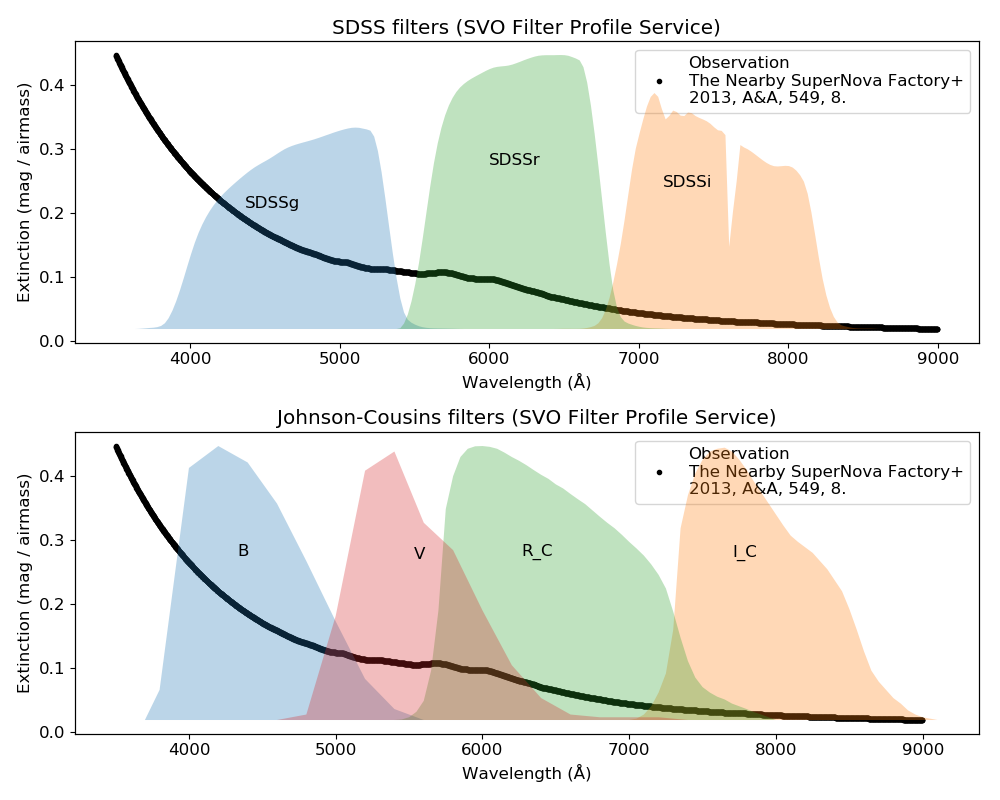
\includegraphics[width=0.9\linewidth]{figs/air-ext-and-filter}
\caption{The atmospheric extinction as a function of wavelength at Mauna Kea, \textit{based on some 4285 standard star spectra obtained on 478 nights spread over a period of 7 years obtained by the Nearby SuperNova Factory using the SuperNova Integral Field Spectrograph.} (excerpt from The Nearby SuperNova Factory+ 2013, A\&A, 549, 8). The SDSS and Johnson-Cousins filters' filter profiles are overplotted.}
\label{fig:air-ext-and-filter}
\end{figure}

Consider an object with spectrum $ S_0(\lambda) $ is at an airmass of $ X $ and underwent atmospheric extinction described by optical depth of $ \tau(\lambda) $. The magnitude at filter with profile $ f(\lambda) $ (say the filter has non-zero profile at $ \lambda \in (\lambda_1, \lambda_2) $) will have the following Pogson's relation:
\begin{equation}
  m_f - m_{0f}
    = -2.5 \lg
      \qty( \frac{\int_{\lambda_1}^{\lambda_2} S_0(\lambda) f(\lambda) e^{-\tau(\lambda) X} d\lambda}
      {\int_{\lambda_1}^{\lambda_2} S_0(\lambda) f(\lambda) d\lambda} ) ~.
\end{equation}
Here $ e^{-\tau(\lambda) X} $ is actually an approximation of $ e^{\int -\tau(\lambda) dX} $. Using Taylor expansions, $ e^{-\tau(\lambda) X} \approx 1 - \tau(\lambda) X $ and $ \lg (1 - A) \approx - A / \ln 10 $, 
\begin{equation}
\begin{aligned}
    m_f - m_{0f} 
    &\approx -2.5 \lg 
      \qty( 1 - \frac{\int_{\lambda_1}^{\lambda_2} S_0(\lambda) f(\lambda) \tau(\lambda) d\lambda}
        {\int_{\lambda_1}^{\lambda_2} S_0(\lambda) f(\lambda) d\lambda} X ) 
    \approx \frac{2.5}{\ln 10} 
      \frac{\int_{\lambda_1}^{\lambda_2} S_0(\lambda) f(\lambda) \tau(\lambda) d\lambda}
            {\int_{\lambda_1}^{\lambda_2} S_0(\lambda) f(\lambda) d\lambda} X ~.
\end{aligned}  
\end{equation}

Remembering $ I = I_0 e^{-\tau X} $, we have $ \Delta m = -2.5 \lg (I / I_0) = 1.086 \tau X $. Then the $ y $-axis of \cref{fig:air-ext-and-filter} is $ \sim 1.1 \tau $, so you can roughly understand that the $ y $-axis of the figure is similar to $ \tau $. Therefore, $ \tau X \ll 1 $ is reasonable. In cases such as short wavelength (shorter than B/g) and high airmass observation, this assumption may break down. The error due to the approximation, however, may not be severe compared to other error sources (e.g., changing weather). 

Now we want to further assume that, $ \tau(\lambda) \approx c_1 + c_2 \lambda $ within the wavelength range of $ (\lambda_1, \lambda_2) $. This is similar to approximating the black markers in \cref{fig:air-ext-and-filter} within each filter as a line because its y-axis is nothing but $ 1.1 \tau $. Then
\begin{equation}
  m_f - m_{0f} 
    \approx 2.5 
    \qty (c_1 + c_2\frac{\int_{\lambda_1}^{\lambda_2} S_0(\lambda) f(\lambda) \lambda d\lambda}
      {\int_{\lambda_1}^{\lambda_2} S_0(\lambda) f(\lambda) d\lambda} ) X ~.
\end{equation}
If the filter is fixed (e.g., V-band or SDSS $ \mathrm{g'} $ filter, etc), the only unknown thing in the second term in the parenthesis is $ S_0(\lambda) $, i.e., the spectral shape. If it is a black body spectrum, it is true that the spectral shape has a one-to-one relationship with the color index\footnote{This is not strictly true. For example, at temperatures between $ T = \SI{15000}{K} $ and $ \SI{40000}{K} $, the color indices are nearly constant as $ \mathrm{B - V} = -0.20 $ and $ -0.30 $. Furthermore, color index is not one-to-one with temperature between 30,000 and 35,000 K, i.e., differemt temperature (different $ S(\lambda) $) can have the same color index. This happens because filter profile is not ``flat'' as a function of $ \lambda $.}.
Even if it is not a perfect black body, it is reasonable to assume the spectral shape, $ S_0(\lambda) $, and color index, $ C $, have \textit{nearly} one-to-one relationship. Thus, $ C $ is an indicator of $ S_0(\lambda) $, so the second term is roughly a function of $ C $, say $ c_2 \tilde{S}(C) $. The final assumption we make here is that the second term is $ c_2 \tilde{S} (C) \approx c_3 + c_4 C $ as the first-order approximation. Here $ c_3 $ and $ c_4 $ depends on the \textit{filter} profile, but not on the spectral shape, under our simplifying assumptions. We denote them with subscript $ f $ which means that filter:
\begin{equation}\label{key}
  m_f - m_{0f} 
  \approx 2.5 (c_1 + c_{3f} + c_{4f} C) X 
  \equiv k_f' X + k_f'' CX
\end{equation}
 These are the origins of $ k_f' $ and $ k_f'' $ in \cref{eq: std}.

To illustrate the result, I used the SDSS filter system as shown in \cref{fig:air-ext-bbrad} and calculated how much magnitude extinction happens depending on the black body temperature:

\begin{table}[ht!]
\centering
  \begin{tabular}{c||ccc}
  Temperature  & $ m_\mathrm{g'} - m_\mathrm{0 g'} $ & $ m_\mathrm{r'} - m_\mathrm{0 r'} $ & $ m_\mathrm{i'} - m_\mathrm{0 i'} $ \\
  \hline
  $ \SI{3000}{K} $  & $ \m{0.142} $ & $ \m{0.081} $ & $ \m{0.034} $ \\
  $ \SI{6000}{K} $  & $ \m{0.158} $ & $ \m{0.084} $ & $ \m{0.035} $ \\
  $ \SI{20000}{K} $ & $ \m{0.171} $ & $ \m{0.087} $ & $ \m{0.036} $ \\
  \end{tabular}
\end{table}

\begin{figure}[ht!]
\centering
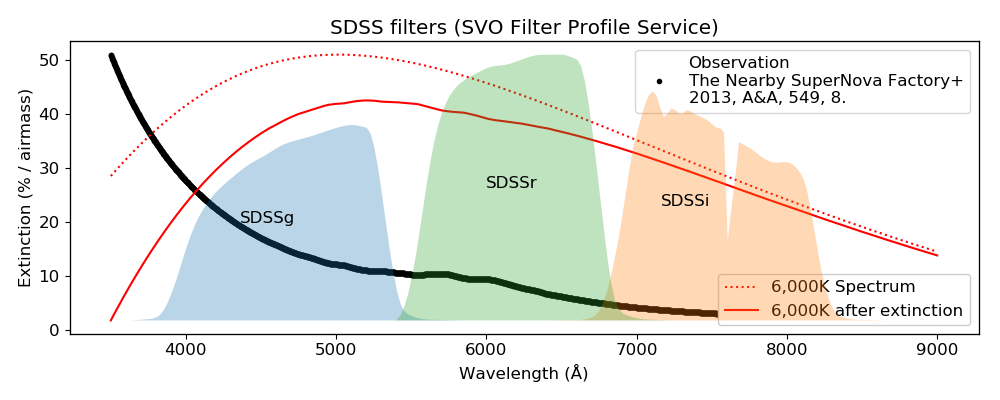
\includegraphics[width=0.9\linewidth]{figs/air-ext-bbrad}
\caption{A black body radiation spectrum ($ T = \SI{6000}{K} $) before and after the extinction at SDSS bands. Note that the y-axis is changed to \% per airmass (cf. \cref{fig:air-ext-and-filter}) by $ 10^{-0.4 \Delta m} $.}
\label{fig:air-ext-bbrad}
\end{figure}

As can be seen, the extinction is stronger for high temperature objects (lower color index), so likely $ k_f'' < 0 $. The difference of extinction between the objects gets smaller as we look at longer wavelength. Thus, $ k_f'' \sim 0 $ except for B or u filters.

These facts can be understood intuitively. The higher the temperature the spectrum will have more fraction of energe at shorter wavelength. Considering that the atmospheric extinction is stronger at shorter wavelength (see black markers in \cref{fig:air-ext-bbrad}), high termperature object will get more ``penalty'' when it comes into the atmosphere. That is why high temperature object is more strongly extincted. But as can be seen, the extinction gets nearly constant at wavelengths of r and i bands. Then this effect will get weaker and that is the reason for smaller discrepancy in $ \Delta m $ values at longer wavelength.

SmithJA+ (2002, AJ, 123, 2121) determined the coefficients for SDSS filters at 1.0 m Ritchey--Chr\'{e}tien telescope at the USNO Flagstaff Station, from the observations in 1998--2000:
\begin{table}[ht!]
\caption{The extinction coefficients of SDSS from SmithJA+ (2002, AJ, 123, 2121).}
\label{tab: SDSS ext}
\centering
  \begin{tabular}{c||lllll}
  Parameter  & u$ ' $ & g$ ' $ & r$ ' $ & i$ ' $ & z$ ' $ \\
  \hline
  $ k_f' $ & $ > +0.5 $ & $ +0.20 \pm 0.05 $ & $ +0.10 \pm 0.05 $ & $ +0.05 \pm 0.05 $ & $ +0.05 \pm 0.05 $\\
  $ k_f'' $ method 1 
    & $ -0.021 \pm 0.003 $
    & $ -0.016 \pm 0.003 $ 
    & $ -0.004 \pm 0.003 $
    & $ +0.006 \pm 0.003 $ 
    & $ +0.003 \pm 0.003 $ \\
  $ k_f'' $ method 2
    & $ -0.032 $ 
    & $ -0.015 $
    &  $ 0.000 $
    & $ +0.005 $
    & $ +0.006 $
  \end{tabular}
\end{table}

The $ k_f' $ value fluctuates much for each night (see Fig 6 of the original publication), so I just took representative values from visual inspection. The $ k_f'' $ values were obtained by two independent pipelines, \texttt{superExcal} (method 1) and \texttt{solve\_network} (method 2). Both are quite consistent except for the u filter.


%Atmosphere diminishes the flux of the object. For an optical depth of $ \tau $, an object with initial flux $ I_0 $ will be observed as $ I = I_0 e^{-\tau} $ and its magnitude will be increased (because flux is decreased) by $ \Delta m = -2.5 \lg (I / I_0) = \frac{2.5}{\lg e} \tau = 1.086 \tau $. But $ \tau = \int n \sigma dl $ for the number density of particles $ n $, the extinction cross-section $ \sigma $, and traveling distance $ l $. The total traveling distance, $ L $, is $ L_0 / \cos z = L_0 X $ where $ X $ is the airmass. Thus, a simple approximation that $ \tau \propto L $ will result in $ \Delta m \propto X $. 

%The real story is more complicated: This extinction is of course wavelength-dependent (\cref{fig:air-ext-and-filter}). The black markers show the extinction magnitude per airmass. At zenith, $ X = 1 $ by definition, so this means that $ \Delta m \sim \m{0.2} $ at $ \lambda = \SI{4000}{\AA} $ but is $ \Delta m \ll \m{0.1} $ for $ \lambda = \SI{8000}{\AA} $. Therefore, the extinction is not simply proportional to $ X $, but the proportionality is a function of wavelength.

%\begin{thm}[Atmospheric Extinction: 1st Order]
%The extinction due to the atmosphere has the following 1st order term:
%\begin{equation*}
%  \Delta m(\lambda) = k'(\lambda) X ~,
%\end{equation*}
%where $ k'(\lambda) $ is the first-order extinction coefficient and is a function of wavelength $ \lambda $. In photometry, we are dealing with filters rather than each single wavelength, so normally we denote 
%\begin{equation}\label{eq: air-ext 1st ord}
%  \Delta m_f = k_f' X ~.
%\end{equation}
%\end{thm}
 

%Consider a black body spectrum is underwent this atmospheric extinction: \cref{fig:air-ext-bbrad}. The extinction is of course a function of wavelength. 

%In photometry, we are interested in the total number of photons \textit{after} multiplied with the filter profile: $ \int_{\lambda_1}^{\lambda_2} S(\lambda) f(\lambda) d\lambda $ where $ S(\lambda) $ is the spectrum and $ f(\lambda) $ is the filter profile. Thus, the magnitude change before and after the atmospheric extinction is, if the extinction is $ E(\lambda) $,
%\begin{equation}
%  \Delta m = 
%    -2.5 \lg \qty (\frac{\int_{\lambda_1}^{\lambda_2} E(\lambda) S(\lambda) f (\lambda) d\lambda}{\int_{\lambda_1}^{\lambda_2} S(\lambda) f(\lambda) d\lambda} )
%\end{equation} 
%Because it contains a ratio of the integration, it is not simple to calculate $ \Delta m $. From target to target, what changes is, except for the airmass (Note that $ E(\lambda) = e^{-\tau} \propto \sim e^X $), the $ S(\lambda) $. Thus, $ \Delta m = \Delta m (X, S) $. For a black body, this is a function of the temperature, and the temperature has (roughly) one-to-one counterpart of the color index. Thus, if the spectral shape is assumed as black body, we can write $ \Delta m = \Delta m (X, C) $ where $ C $ is the true color index. Even if it is not a black body, it is sufficient if the spectral shape and color index have \textit{nearly} one-to-one relationship. The extinction due to the spectral shape should also be proportional to the airmass to the first order approximation. Thus, as an approximation, we add a term proportion to $ CX $ to  \cref{eq: air-ext 1st ord}:

%\begin{thm}[Atmospheric Extinction: 2nd Order]
%The extinction due to the atmosphere is:
%\begin{equation}
%  \Delta m(\lambda) = k'(\lambda) X + k''(\lambda) C X ~,
%\end{equation}
%where $ k''(\lambda) $ is the second order atmospheric extinction coefficient.
%In photometry, we are dealing with filters rather than each single wavelength, so normally we denote 
%\begin{equation}\label{eq: air-ext 2nd ord}
%  \Delta m_f = k_f' X + k_f'' C X ~.
%\end{equation}
%\end{thm}

The atmospheric extinction coefficients $ (k_f',\, k_f'') $ all change as a function of time. We just hope they are reasonably constant during our observation of our targets and standard stars. From experience, we know $ k_f'' $ is almost very small for filters longer than u or B-band, but is not necessarily ignorable because $ k_f'' XC $ might be larger than the accuracy you want to obtain. 

\begin{ex}[Ignoring the Second Order Extinction Term]
Consider an observation at $ X = 2 $ of $ C = 0.2 $ star. If you ignore the second order extinction term, you are making $ k_f'' XC = 0.4 k_f'' $ of uncertainty. According to \cref{tab: SDSS ext}, this is most likely smaller than 0.01 magnitude. 

The Sun has $ C = \mathrm{g' - r'} \sim 0.5 $, and the error becomes $ 1.0 k_f'' $ and it is $ < \m{0.01} $ only for riz bands.

The red M0 stars have $ C = \mathrm{g' - r'} \lesssim 1.5 $ and the error is now $ 3.0 k_f'' $. The accuracy of $ \m{0.01} $ can be achieved in riz bands, but risky.
\end{ex}

The calculation above is only for SDSS observatory at altitude of 2.3 km. But fortunately, BuchheimB (2005, SASS, 24, 111) found that the $ k_f'' \lesssim 0.005 $ for V band even at many low-altitude observatories (including Bochum observatory at altitude 200 m, Vainu Bappu Observatory at altitude 700 m), so likely we expect the correction from the second-order extinction term is small enough.


\subsection{Transformation Coefficient}
The sensitivity of the optics is also a function of $ \lambda $. The argument is identical to atmospheric extinction, but there is no $ X $ (similar parameter will be something like the optical depth of materials blocking CCD pixel, but that should be a device-dependent constant). Then the same logic leads us to the conclusion that there should be a color term which tunes the final output of the CCD count, and that is the $ k_f C $ (``transformation'') term.

The transformation coefficient, which I denoted $ k_f $, is fortunately nearly constant for the given device. Warner argues that it is enough to update $ k_f $ (Warner uses notation of $ T_f $) value only about 2--4 times a year, unless you physically changed the device elements (e.g., filter, CCD, lens, etc). Moreover, from experience, we know that this is nearly zero: $ |k_f| \lesssim 0.1 $. Many cases $ |k_f| \lesssim 0.01 $. Since the range of color indices are $ \mathrm{max}(\Delta C) \lesssim \m{1} $, we have $ |k_f C| \lesssim 0.1 $, and in many cases, $ |k_f C| \lesssim 0.01 $.


\section{Differential Photometry}
Now that we justified the usage of \cref{eq: std}, let's find the cases of application. The simplest case is the \textit{differential photometry}. 

If there are many celestial objects (of course including your target) in the field of view with known standard magnitudes, we can use them as standard stars. Although there can be variable stars and galaxies\footnote{Galaxies can have spectra significantly different from those of black bodies. Therefore, the coefficients $ k_f $ and $ k_f'' $, which are approximations of spectral shape (i.e., not $ k_f' $), should be different from those derived from standard \textit{stars}, which are black bodies. But mostly this effect is not serious because, as we discussed before, both $ k_f C $ and $ k_f'' X C $ terms are anyway very small. For this reason, people use $ k_f $ and $ k_f'' $ derived from standard stars for their target galaxies (or any non-black body like spectra). If you really worry about this, you must conduct spectroscopic observation, not broad-band photometry.}, if most of the objects with known magnitudes are non-variable stars, those \textit{outliers} will be smoothed out. Thus, we just assume all the celestial objects in the field of view with known standard magnitudes as ``standard stars''. 

This technique is very widely used in variable star and asteroidal light curve observations. This is widely used than normal (absolute) photometry, because it is annoying and difficult to observe standard stars at different airmasses while observing your target, which requires telescope time and human labor. In asteroidal science, even single-filter differential photometry is frequently used. 


\subsection{Multi-Filter Differential Photometry}
When we have more than one filter observation, we can get do the photometry in a rather complete way. As a simple example, consider a 2-filter observation. Rearranging \cref{eq: std} gives
\begin{equation}
  M_f - m_f = z_f - k_f' X + (k_f - k_f''X) C ~.
\end{equation}
In the same FOV, they should have almost identical airmass and zero point. If we observe the same field with filter $ x $ (at airmass of $ X_x $) and $ y $ (at airmass of $ X_y $), and denote $ C_{xy} = M_x - M_y $,
\begin{equation}
\begin{cases}
  M_x - m_x &= (z_x - k_x' X_x) + (k_x - k_x''X_x) C_{xy} = a_x + b_x C_{xy} \\
  M_y - m_y &= (z_y - k_y' X_y) + (k_y - k_y''X_y) C_{xy} = a_y + b_y C_{xy} 
\end{cases}
\end{equation}
Note here that, for field stars with known standard magnitudes, $ M_x $, $ M_y $, and thus $ C_{xy} = M_x - M_y $ should all be known for $ N $ ``standard stars'' in the image. The $ m_x $ and $ m_y $ are direct results from the photometry, so these should also be known from the image. Also, the values involved in $ a $ and $ b $ factors, there is no color-term, i.e., they should be identical for all the objects in the image\footnote{Of course we are assuming the coefficients, i.e., weather and CCD properties are constant over the time of $ x $ and $ y $ image exposures.}. Then what we have to determine are the two sets of constants, $ (a_x, b_x) $ and $ (a_y, b_y) $. 

If we plot $ M_x - m_x $ as ordinate and $ C_{xy} $ as abscissa for $ N $ field stars (the ``standard stars''), the y intercept is $ a_x $ and the slope is $ b_x $. Same goes for the $ y $ filter. So  $ (a_x, b_x) $ and $ (a_y, b_y) $ are determined with the uncertainties.

Then for the target, what we have to do is to solve
\begin{equation}
\begin{cases}
  M_x^\mathrm{target} - m_x^\mathrm{target} &= a_x + b_x C_{xy}^\mathrm{target} \\
  M_y^\mathrm{target} - m_y^\mathrm{target} &= a_y + b_y C_{xy}^\mathrm{target}
\end{cases}
\end{equation}
or since $ C_{xy}^\mathrm{target} = M_x^\mathrm{target} - M_y^\mathrm{target} $,
\begin{equation}
  C_{xy}^\mathrm{target} = \frac{m_x^\mathrm{target} - m_y^\mathrm{target} + (a_x - a_y)}{1 - (b_x - b_y)} ~.
\end{equation}
Putting this back to the original equation,
\begin{equation}\label{eq: 2-filter diff phot sol}
\begin{cases}
  M_x^\mathrm{target}
    = m_x + a_x + b_x \frac{m_x^\mathrm{target} - m_y^\mathrm{target} + (a_x - a_y)}{1 - (b_x - b_y)} \\
  M_y^\mathrm{target}
    = m_y + a_y + b_y \frac{m_x^\mathrm{target} - m_y^\mathrm{target} + (a_x - a_y)}{1 - (b_x - b_y)}
\end{cases}
\end{equation}
Now we have the standard magnitude of the target in both $ x $ and $ y $ filters.

What if we have more than 2 filters, say $ x $, $ y $, and $ z $? Solve for $ x $ and $ y $ as above by using $ (a_x, b_x) $. Then solve for $ y $ and $ z $, but this time using color as $ C_{yz} $, not $ C_{xy} $, using $ (a_x', b_x') $. Theoretically $ a_x = a_x' $, because there is no color term. However, $ b_x \neq b_x' $, because $ k_y'' $ is defined for $ C_{xy} $ for the first case, but it is defined for $ C_{yz} $ for the second case. In reality, because what we get is only the best-fit values with uncertainties, $ a_x $ and $ a_x' $ can also be different (likely within certain amount of error-bar).

\subsection{Single-Filter Differential Photometry}
Sometimes 
\begin{enumerate}
\item we don't have multi-filter (also called the ``multi-color'') observation data of the  target, or
\item the linear fit to $ M - m $ VS $ C_{xy} $ is not possible because there are only few stars and/or narrow color range. 
\end{enumerate}
For the first case, although we can get $ (a_x, b_x) $, we don't know the $ C_{xy} $ (mathematically identical to state that we don't have parameters with subscript $ y $ to plug into \cref{eq: 2-filter diff phot sol}). For the second case, it is just impossible to get $ (a_x, b_x) $. Then we have to assume a little more and do a \textit{single-filter} differential photometry.

This is used in the cases when $ b_f C = (k_f - k_f'' X) C $ is smaller than the photometric accuracy we seek for. This happens, e.g., when the uncertainty of $ M_f $ is larger than $ b_f C $. Then we simply drop that term because the uncertainty due to this term will be smaller than the final uncertainty. Thus,
\begin{equation} \label{eq: 1-filter diff phot}
  M_f \approx m_f + (z_f - k_f' X) = m_f + Z_f ~.
\end{equation}

In the same FOV, they should have almost identical airmass and zero point. Therefore, under the same filter $ f $, we have $ Z_f \simeq \mathrm{const} $ for all the objects (of course including our target) in the same CCD image. This is the different point from previous multi-filter observation, and this happens because we ignored color. What we have to do here is to find that constant by plotting $ M_f $ and $ m_f $ of the field objects, and fit a linear line. In the process of finding the $ Z_f $ (sometimes people call it just ``zero point'', although rigorously the zero point should be $ z_f $), one should note that the slope must be unity. For this reason sometimes we fit a line while \textit{fixing the slope as unity}. 

If we set the slope as a free parameter, as well as the zero point, and if the best-fit slope deviated far from 1, that means (1) many field objects are variable or highly non-blackbody-like galaxies so that they are not suitable as ``standard stars'' and the basic assumptions of \cref{eq: std} break down, (2) the color term is not actually negligible so \cref{eq: 1-filter diff phot} is not a good approximation, (3) catalog $ M_f $ suffer from unknown uncertainties or systematic errors so the catalog value is not reliable, (4) $ m_f $ was measured incorrectly, (5) many other possibilities. 


\section{Photometry Using Standard Stars}
The idea is similar to multi-filter differential photometry, but we use the real standard stars. Except for few fields of standard stars (where many standard stars are located within small FOV), \textit{there is only one single standard star in a CCD image}. This makes it different from the differential photometry.

Consider a standard star with ID $= i $ is observed for $ N_i $ times, and denote each observation as $ j $ $ (j = 1, \cdots, N_i) $, and write the parameters of \cref{eq: std} as $ M_{f, i} $, $ C_{i} $ ($ M $ and $ C $ are fixed values for a standard star, so no $ j $ is needed), $ m_{f, i}^{(1)} $, $ X_{f, i}^{(1)} $, etc. We here assume the zero point, $ z_f $, and the coefficients $ k_f $, $ k_f' $, and $ k_f'' $ are almost constant over the night\footnote{Even SDSS standard stars were also observed and analyzed under this assumption. See SmithJA (2002, AJ, 123, 2121)}. Then
\begin{equation}
\begin{cases}
  M_{f, i} - m_{f, i}^{(1)}
    &= z_f + k_f' X_{f, i}^{(1)} + k_f'' X_{f, i}^{(1)} C_{i} + k_f C_{i} \\
  M_{f, i} - m_{f, i}^{(2)}
    &= z_f + k_f' X_{f, i}^{(2)} + k_f'' X_{f, i}^{(2)} C_{i} + k_f C_{i}
\end{cases}
\end{equation}
for the first two observations of the same standard star (ID $= i $) at filter $ f $. Subtracting two,
\begin{equation}
  \Delta m_{f, i}^{(1, 2)} 
    = (k_f' + k_f'' C_i) \Delta X_{f, i}^{(1, 2)} 
  \quad\rightarrow\quad
  \qty( \frac{\Delta m }{\Delta X} )_{f, i}^{(1, 2)}
    = k_f' + k_f'' C_i ~.
\end{equation}
Of course $ \Delta m_{f, i}^{(1, 2)}  = m_{f, i}^{(1)} - m_{f, i}^{(2)} $ and $ \Delta X_{f, i}^{(1, 2)}  = X_{f, i}^{(1)} - X_{f, i}^{(2)} $. 

Therefore, if we plot $ \qty ( \frac{\Delta m }{\Delta X} )_{f, i} $ as a function of color $ C_i $ of the standard stars with different color indices (colors of them are all known), the linear fit will give intercept of $ k_f' $ and slope of $ k_f'' $. For star $ i $, we have $ N_i $ observations, so we have $ \binom{N_i}{2} = N_i (N_i - 1) / 2 $ points at the single $ C_i $ value. If we have $ N $ standard stars of wide color range, we can have $ N \sum_i \binom{N_i}{2} $ points to fit the linear line.